% Section content template for individual Educative lessons
% This file contains the actual content for a specific section
% Generated from Educative API section content

% Section: System Design: YouTube
% Section ID: 5360542734090240
% Section Slug: system-design-youtube
% Generated: 2025-12-07T22:36:32.993052

\subsection{What is YouTube?}\label{gCncpFZG2QPyUomxBshg8}
\\
YouTube is a popular video streaming service where users upload, stream, search, comment, share, and like or dislike videos. Large businesses as well as individuals maintain channels where they host their videos. You Tube allows free hosting of video content to be shared with users globally. You
Tube is considered a primary source of entertainment, especially among young people, and as of 2022, it is listed as the second-most viewed website after Google by Wikipedia(See https://en.wikipedia.org/wiki/List\_of\_most\_visited\_websites).

\begin{figure}[htbp]
 \centering
 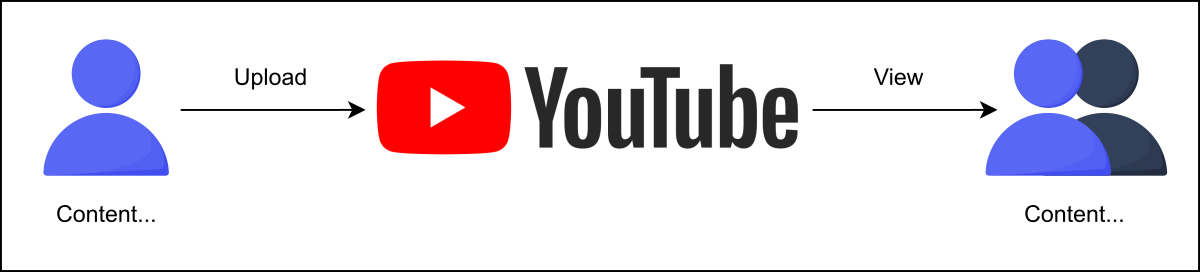
\includegraphics[width=0.5\textwidth]{Images/chapter_26/section_5360542734090240/4912187317813248.png}
 \caption{A depiction of a content creator uploading a video to YouTube that is streamed by many viewers}
\end{figure}

\subsection{YouTube's popularity}\label{kIWX_heYkuuyB8-RSXV8i}
\\
Some of the reasons why YouTube has gained popularity over the years include the following reasons:

\begin{itemize}
\item
\protect\phantomsection\label{Sk80LNz4fVA1c9rUgUS4P}
\textbf{Simplicity}: YouTube has a simple yet powerful interface.
\item
\protect\phantomsection\label{wGUQ2Jx0lwQguYU7bgax4}
\textbf{Rich content}: Its simple interface and free hosting has attracted a large number of content creators.
\item
\protect\phantomsection\label{7Uu83EldY1zvMs08N6ypt}
\textbf{Continuous improvement}: The development team of YouTube has worked relentlessly to meet scalability requirements over time. Additionally, Google acquired YouTube in 2007, which has added to its credibility.
\item
\protect\phantomsection\label{GoeGD_Pg2eNiHgUyrAEYI}
\textbf{Source of income}: YouTube coined a partnership program where it allowed content creators to earn money with their viral content.
\end{itemize}
\\
Apart from the above reasons, YouTube also partnered up with well-established market giants like CNN and NBC to set a stronger foothold.

\subsection{YouTube's growth}\label{7uu0w8L-VylT4NJRY495Z}
\\
Let's look at some interesting statistics about YouTube and its popularity.
\\
Since its inception in February 2005, the number of YouTube users has multiplied. As of now, there are more than 2.5 billion monthly active users of YouTube. Let 's take a look at the chart below to see how YouTube users have increased in the last decade.

\textbf{YouTube's Yearly User Growth}

\textit{\small [Chart data presented in table format]}

\begin{table}[htbp]
\centering
\small
\adjustbox{max width=\textwidth}{
\begin{tabular}{|p{0.475\textwidth}|p{0.475\textwidth}|}
\hline
\textbf{Year} & \textbf{Monthly Active Users} \\
\hline
\hline
2012 & 0.8 \\
\hline
2013 & 1 \\
\hline
2014 & 1.1 \\
\hline
2015 & 1.2 \\
\hline
2016 & 1.4 \\
\hline
2017 & 1.5 \\
\hline
2018 & 1.8 \\
\hline
2019 & 2 \\
\hline
2020 & 2.3 \\
\hline
2021 & 2.6 \\
\hline
\end{tabular}
}
\caption{Increase in monthly active users of YouTube per year}
\label{tab:chart}

\textit{\small Note: Values are in Billion}
\end{table}

YouTube is the second most-streamed website after Netflix. A total of 694,000 hours of video content is streamed on YouTube per minute.
\\
Let's evaluate your understanding of the building blocks required in the design of YouTube. Based on the functional and nonfunctional requirements given below, identify three key building blocks needed to curate the design of YouTube.

\begin{itemize}
\item
\textbf{Functional requirements:}

\begin{itemize}
\item
Stream videos
\item
Upload videos
\item
Search videos according to titles
\item
Like and dislike videos
\item
Add comments to videos
\item
View thumbnails
\end{itemize}
\item
\textbf{Nonfunctional requirements:}

\begin{itemize}
\item
High availability
\item
Scalability
\item
Good performance
\end{itemize}
\end{itemize}
\\
You should focus on the building blocks required for \textbf{back-end storage and efficient data transmission} to end users. Please also specify the reason(s) behind the selection of a building block.

\textbf{Question:}

List three key building blocks necessary to design a system like YouTube.

\textbf{Reference Answer:}

The three key building blocks are:

\begin{itemize}
\tightlist
\item
Databases are required to store the metadata of videos, thumbnails, comments, and user-related information.
\item
Blob storage is important for storing all videos on the platform.
\item
A CDN effectively delivers content to end users, reducing delay and burden on end-servers.
\end{itemize}

Let's understand how to design YouTube in the next lessons.

\subsection{How will we design YouTube?}\label{mt8IyDQRiQlNRwxW7F9WM}
\\
We've divided the design of YouTube into five lessons:

\begin{enumerate}
\item
\protect\phantomsection\label{e-ITJ88Ucdv36kq-0SJsS}
\href{https://www.educative.io/courses/grokking-the-system-design-interview/requirements-of-youtubes-design}{\textbf{Requirements}}: This is where we identify the functional and non-functional requirements. We also estimate the resources required to serve millions of users each day. This lesson answers questions like how much storage space YouTube will need to store 500 hours of video content uploaded to YouTube per minute.
\item
\protect\phantomsection\label{jkga7-cAdHBFqWjtc7lv4}
\href{https://www.educative.io/courses/grokking-the-system-design-interview/design-of-youtube}{\textbf{Design}}: In this lesson, we explain how we'll design the YouTube service. We also briefly explain the API design and database schemas. Lastly, we will also briefly go over how YouTube's search works.
\item
\protect\phantomsection\label{3wzNipD02fiCfBVHR6K_4}
\href{https://www.educative.io/courses/grokking-the-system-design-interview/evaluation-of-youtubes-design}{\textbf{Evaluation}}: This lesson explains how YouTube is able to fulfill all the requirements through the proposed design. It also looks at how scaling in the future can affect the system and what solutions are required to deal with scaling problems.
\item
\protect\phantomsection\label{qwwKCVkJSbf_0dTuNYKLV}
\href{https://www.educative.io/courses/grokking-the-system-design-interview/the-reality-is-more-complicated}{\textbf{Reality is more complicated}}: During this lesson, we'll explore different techniques that YouTube employs to deliver content effectively to the client and avoid network congestions.
\item
\protect\phantomsection\label{3Ic8OOsv03Of16U1-JXkK}
\href{https://www.educative.io/courses/grokking-the-system-design-interview/quiz-on-youtubes-design}{\textbf{Quiz}}: We reinforce major concepts we learned designing YouTube by considering how we could design Netflix's system. Our discussion on the usage of various building blocks in the design will be limited since we've already explored them in detail in the \href{https://www.educative.io/courses/grokking-the-system-design-interview/introduction-to-building-blocks-for-modern-system-design}{building blocks} chapter.
\end{enumerate}

% End of section content